\chapter{THIẾT KẾ BỘ TRUYỀN ĐAI THANG}
    \section*{2.0. THÔNG SỐ KỸ THUẬT BỘ TRUYỀN ĐAI THANG}
        \begin{itemize}
            \item Công suất trục động cơ: $P_{I} = 3.07(kW)$.
            \item Tỉ số truyền bộ truyền: $u_{d} = 2$.
            \item Số vòng quay bánh dẫn: $n_{I} = 720(rpm)$.
            \item Momen xoắn: $T_{I} = 40.72(N.m)$. 
        \end{itemize}
    \section{CHỌN LOẠI ĐAI VÀ TIẾT DIỆN}
        \hspace*{0.6cm}Kích thước bánh đai thang thường được chia làm 7 loại chính Z, A, B, C, D, E. Với bảng chọn dạng đai phụ thuộc vào công suất truyền của trục và vận tóc góc trục được thiết kế.\\
        \hspace*{0.6cm}Dựa vào bảng 4.3 tài liệu tham khảo \cite{gtctm}, với công suất trục động cơ $P_{I} = 3.07(kW)$ và số vòng quay bánh dẫn $n_{I} = 720(rpm)$, ta chọn được loại đai thang:\\  
        \begin{figure}[H]
            \centering
            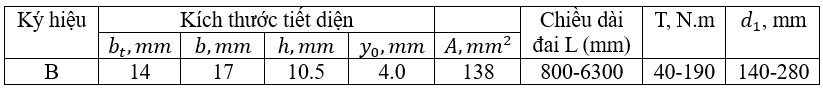
\includegraphics[width=1\textwidth]{pictures/belt.png}
            \caption{Chọn loại đai}
        \end{figure}

    \section{XÁC ĐỊNH CÁC THÔNG SỐ BỘ TRUYỀN}
        \subsection{Xác định sơ bộ đường kính bánh đai nhỏ}
            \hspace*{0.6cm}Đường kính bánh đai nhỏ $d_1 = 1.2d_{min}$ với $d_{min} = 125$. Chọn sơ bộ theo tiêu chuẩn $d_1 = 160mm$\\
            \hspace*{0.6cm}Vận tốc đai sơ bộ trên bánh đai dẫn:
                $$v_1 = \frac{\pi d_1 n_1}{60000} = \frac{\pi \cdot 160 \cdot 720}{600000} = 6.03(mm/s)$$ \\
            $\Rightarrow$ Vậy thỏa điều kiện $v < 25 (m/s)$, ta tiếp tục tính toán với đai thường.
        \subsection{Tính chính xác đường kính 2 bánh đai}
            \begin{itemize}
                \item Chọn hệ số trượt tương đối $\xi = 0.01$.
                \item Theo công thức 4.10 tài liệu tham khảo \cite{gtctm}, ta có tỉ số truyền bộ truyền đai:
                    \begin{equation}
                        u = \frac{d_2}{d_1(1 - \xi)}
                    \end{equation}
                    $$\Rightarrow d_2 = u \cdot d_1(1 - \xi) = 2 \cdot 160(1 - 0.01) = 316.8 (mm)$$
                    Theo tiêu chuẩn ta chọn $d_2 = 315(mm)$.
                \item Tính lại đường kính bánh đai nhỏ:
                    $$d_1 = \frac{d_2}{u \cdot (1 - \xi)} = \frac{315}{2 \cdot (1 - 0.01)} = 159.09(mm)$$
            \end{itemize}
        \subsection{Chọn khoảng cách trục a và chiều dài đai L}
            \begin{itemize}
                \item Chọn sơ bộ a theo bảng trang 166 tài liệu tham khảo \cite{gtctm}, với $u = 2$, ta chọn $a = 1.2 \cdot d_2 = 1.2 \cdot 315 = 378(mm)$.
                \item Chiều dài đai được tính theo công thức:
                    \begin{equation}
                        L = 2a + \frac{\pi(d_1 + d_2)}{2} + \frac{(d_2 - d_1)^2}{4a} 
                    \end{equation}
                    $$\Rightarrow L = 2 \cdot 378 + \frac{\pi(159.09 + 315)}{2} + \frac{(315 - 159.09)^2}{4 \cdot 378} = 1516.78(mm)$$
                    Theo tiêu chuẩn ở bảng 4.13 tài liệu tham khảo \cite{tltk1}, ta chọn $L = 1600 (mm)$.\\
                \item Từ đó ta tính chính xác lại khoảng cách trục a theo công thức 4.6 tài liệu tham khảo \cite{tltk1}:
                    \begin{align}
                        a = \frac{\lambda + \sqrt{\lambda^2 - 8\Delta^2}}{4} = \frac{855.3 + \sqrt{855.3^2 - 8 \cdot 77.95^2}}{4} = 420.42(mm)
                    \end{align}
                    Trong đó:
                    \begin{itemize}
                        \item $\lambda = L - \frac{\pi(d_1 + d_2)}{2} = 1600 - \frac{\pi(159.09 + 315)}{2} = 855.3.$
                        \item $\Delta = \frac{d_2 - d_1}{2} = \frac{315 - 159.09}{2} = 77.95.$
                    \end{itemize}
                \item Kiểm nghiệm khoảng cách trục a theo công thức 4.14 tài liệu tham khảo \cite{tltk1}:
                    \begin{align*}
                        0.55(d_1 + d_2) + h \leq &a \leq 2(d_1 + d_2).\\
                        0.55(159.09 + 315) + 10.5 \leq 42&0.42 \leq 2(159.09 + 315).\\
                        271.25 \leq 42&0.42 \leq 948.18.   
                    \end{align*}
                    \hspace*{0.6cm}Vậy $a = 420.42(mm)$ thỏa điều kiện.
            \end{itemize}
        \subsection{Tính toán vận tốc đai và số vòng chạy đai}  
            \begin{itemize}
                \item Vận tốc bánh dẫn:
                    $$v_1 = \frac{\pi d_{1} n_{I}}{60000} = \frac{\pi \cdot 159.09 \cdot 720}{60000} = 6 (m/s)$$
                \item Vận tốc bánh bị dẫn:
                    $$v_2 = \frac{\pi d_{2} n_{II}}{60000} = \frac{\pi \cdot 315 \cdot 360}{60000} = 5.94 (m/s)$$  
                \item Số vòng chạy đai trong 1 giây:
                    $$i = \frac{v_1}{L} = \frac{6}{1600 \cdot 10^{-3}} = 3.75 < [i]_{\text{đai thang}} = 10 (s^{-1}) $$
                    $\Rightarrow$ Đai thang thỏa điều kiện.
            \end{itemize}
        \subsection{Xác định góc ôm đai trên bánh nhỏ}
            \hspace*{0.6cm}Vì hệ thống truyền động đai của chúng ta có trục chuyển động song song cùng chiều nên góc ôm đai bánh đai nhỏ $\alpha_1$ được tính như công thức 4.7 tài liệu tham khảo \cite{tltk1}:
            $$a_{1} = 180 - \frac{57(d_2 - d_1)}{a} = 180 - \frac{57(315 - 159.09)}{369.17} = 158.75^{\circ}$$
            $\Rightarrow \beta = 180 - \alpha_1 = 21.25^{\circ}$.
    \section{XÁC ĐỊNH SỐ ĐAI}
        \hspace*{0.6cm}Từ công thức 4.16 tài liệu tham khảo \cite{tltk1}, ta có số đai được xác định như sau:
        \begin{equation}
            Z = \frac{P_{I} \cdot K_{d}}{[P_{0}]C_{\alpha}C_{l}C_{u}C_{z}} 
            \label{eq:2.4}
        \end{equation}
        \begin{itemize}
            \item Hệ số ảnh hưởng góc ôm đai:
            $$ C_{\alpha} = 1.24(1 - e^{-\alpha_1/110}) = 1.24(1 - e^{\frac{-158.75}{110}}) = 0.947$$
            \item Hệ số ảnh hưởng chiều dài đai: Với $\frac{l}{l_o} = \frac{1600}{2240} = 0.71$. Tra bảng 4.16, tài liệu tham khảo \cite{tltk1}, ta nội suy được $C_{l} = 0.925$.
            \item Hệ số ảnh hưởng của tỉ số truyền: Với $u_d = 2$. Tra bảng 4.17, tài liệu tham khảo \cite{tltk1} ta nội suy được $C_{u} = 1.12$.
            \item Hệ số ảnh hưởng của tải trọng không đều: Ta chọn sơ bộ $C_z = 0.95$ với giả định $z \in (2 \div 3)$.
            \item Hệ số tải trọng động $K_d = 1$.
            \item Trị số công suất cho phép với đai thang thường: Tra bảng 4.19, tài liệu tham khảo \cite{tltk1} với đai loại B, đường kính bánh nhỏ $d_{1} = 159.09 (mm)$ và vận tốc đai $v = 6 (m/s)$, ta chọn $[P_{0}] = 2 (kW)$. 
        \end{itemize}
        \newpage
        Từ công thức \ref{eq:2.4}, ta có số đai: $$Z = \frac{3.07 \cdot 1}{2 \cdot 0.947 \cdot 0.925 \cdot 1.12 \cdot 0.95} = 1.64$$
        \hspace*{0.6cm}Theo tiêu chuẩn ta chọn $Z = 2$. $\Rightarrow$ Ta chọn $C_z = 0.95$ là hợp lý.
    \section{XÁC ĐỊNH LỰC TRÊN BÁNH ĐAI}
        \subsection{Lực căng trên đai}
            \begin{itemize}
                \item Tổng lực căng đai ban đầu trên cả 3 dây đai:
                $$F_{0} = z \cdot A_0 \cdot [\sigma_0] = 2 \cdot 138 \cdot 1.5 = 414 (N)$$
                Trong đó: đối với đai thang, $\sigma_0 \leq $ 1.5 MPa nên ta chọn $\sigma_0 = 1.5$ MPa.  
                \item Lực căng trên mỗi dây đai:
                $$\frac{F_0}{z} = \frac{414}{2} = 207 (N)$$
                \item Tổng lực vòng có ích trên cả 3 dây đai:
                $$F_t = \frac{1000P_I}{v_1} = \frac{1000 \cdot 3.07}{6} = 511.67 (N)$$
                \item Lực vòng có ích trên mỗi dây đai:
                $$\frac{F_t}{z} = \frac{511.67}{2} = 255.84 \text{(N)}$$
                \item Lực trên nhánh chủ động và nhánh bị động:
                $$F_{1} = F_0 + \frac{F_t}{2} = 414 + \frac{511.67}{2} = 669.84 (N)$$
                $$F_{2} = F_0 - \frac{F_t}{2} = 414 - \frac{511.67}{2} = 158.17 (N)$$
            \end{itemize}
        \subsection{Lực tác dụng lên trục}
            $$F_r \approx 2F_0sin(\frac{\alpha_1}{2}) = 2 \cdot 414 \cdot sin(\frac{158.75}{2}) = 813.8 (N)$$
            \hspace*{0.6cm}Lại có: $F_r = F_1cos(\frac{\beta}{2} - \theta) + F_2cos(\frac{\beta}{2} + \theta)$. $\Rightarrow \theta= 13.23^{\circ}$. 
        \subsection{Ứng suất lớn nhất trong đai}
            \begin{align*}
                \sigma_{max} &= \sigma_1 + \sigma_v + \sigma_{F1} = \sigma_0 + 0.5\sigma_t + \sigma_v + \sigma_{F1} \\
                &= 0.5 \cdot \frac{F_0}{A} + 0.5 \cdot \frac{F_t}{A} + \rho \cdot v^2.10^{-6} + E \cdot \frac{2 \cdot y_0}{d_1}\\
                &= 0.5 \cdot \frac{414}{138} + 0.5 \cdot \frac{511.67}{138} + 1200 \cdot 6^2.10^{-6} + 100 \cdot \frac{2 \cdot 4}{159.09} = 8.43 \text{(MPa)}
            \end{align*}
    \section{XÁC ĐỊNH CHIỀU RỘNG BÁNH ĐAI VÀ ĐƯỜNG KÍNH VÒNG NGOÀI CÁC BÁNH ĐAI}
        \subsection{Chiều rộng bánh đai}
            \hspace*{0.6cm}Chiều rộng bánh đai được tính theo công thức 4.17, tài liệu tham khảo \cite{tltk1}:\\
                $$B = (z - 1)t + 2e = (2 - 1)\cdot 19 + 2 \cdot 12.5 = 44 (mm) $$
            \hspace*{0.6cm}Trong đó, từ bảng 4.21, tài liệu tham khảo \cite{tltk1}:
            \begin{itemize}
                \item $t = 19 (mm)$.
                \item $e = 12.5 (mm)$.
                \item $h_{0} = 4.2 (mm)$.
            \end{itemize}
        \subsection{Đường kính ngoài của bánh đai nhỏ và bánh đai lớn}
            $$d_{a1} = d_1 + 2h_0 = 159.09 + 2 \cdot 4.2 = 167.49 (mm)$$
            $$d_{a2} = d_2 + 2h_0 = 315 + 2 \cdot 4.2 = 323.4 (mm)$$
    \section{TUỔI THỌ ĐAI}
        $$L_h = \frac{{(\cfrac{\sigma_r}{\sigma_{max}})^m.10^7}}{2.3600.i} = \frac{(\cfrac{9}{8.43})^8.10^7}{2 \cdot 3600 \cdot 3.75} = 625.11 \text{ (giờ)}$$
        Trong đó:
        \begin{itemize}
            \item $\sigma_r$ = 9 (MPa) - giới hạn mỏi của đai thang.
            \item m = 8 - chỉ số mũ của đường cong mỏi đối với đai thang.
            \item i = 3.75 $(s^{-1})$ - số vòng chạy của đai trong một giây.
        \end{itemize}
        Vậy với yêu cầu chạy 300 giờ/năm thì phải thay dây đai mỗi: $L_h / L = 625.11 / 300 = 2.08$ (năm).
    \section{BẢNG THÔNG SỐ BỘ TRUYỀN ĐAI}
    \begin{table}[H]
        \centering
        \begin{tabular}{|c|c|c|}
            \hline
            \textbf{Thông số} & \textbf{Ký hiệu} & \textbf{Giá trị} \\ \hline
            Loại đai & \multicolumn{2}{c|}{B} \\ \hline
            Số đai & z & 2 \\ \hline
            Đường kính bánh nhỏ & $d_1$ & 159.09 (mm)\\ \hline
            Đường kính bánh lớn & $d_2$ & 315 (mm)\\ \hline
            Chiều rộng bánh đai & $B$ & 44 (mm)\\ \hline
            Chiều dài đai & $L$ & 1600 (mm) \\ \hline
            Khoảng cách trục & $a$ & 420.42 (mm) \\ \hline
            Góc ôm đai & $\alpha_1$ & $158.75^o$ \\ \hline
            Lực căng đai ban đầu & $F_0$ & 414 (N) \\ \hline
            Lực tác dụng lên trục & $F_r$ & 813.8 (N)  \\ \hline
            Lực vòng có ích & $F_t$ & 511.67 (N) \\ \hline
            Ứng suất lớn nhất & $\sigma_{max}$ & 8.43 (MPa) \\ \hline
            Tuổi thọ đai & $L_h$ & 625.11 (giờ) \\ \hline
        \end{tabular}
        \caption{Bảng thông số bộ truyền đai}
    \end{table}
        
        